This chapter is thematically divided into four sections, for each of which a high-level concept or architecture is proposed, that aims to fulfill the requirements stated in \autoref{sec:problem_analysis:goals_requirements}. Various design options are discussed and the proposed system's novelty in comparison to previous approaches is conclusively outlined.

Throughout this chapter, requirements from \autoref{sec:problem_analysis:goals_requirements} are referenced with the prefixes \textit{\textbf{F-}} and \textit{\textbf{NF-}}, respectively.

\section{Environment Modeling \& State Representation}
\label{sec:concept_design:environment_modeling_state_representation}
As stated in \autoref{sec:problem_analysis:goals_requirements}, a major goal of this thesis is to propose a common way to model and represent dynamic traffic scenes with the purpose of being used for cooperative perception. The following sections present challenges, requirements, design decisions and eventually a holistic concept.

In \autoref{subsec:concept_design:object_level_representation_fusion}, the decision for using high-level fusion is motivated and an overview of information to be included in the proposed model is outlined. In \autoref{subsec:concept_design:principle_of_dynamic_world_modeling}, modeling principles to be respected during the design phase are presented. Then, a basic structure / framework is proposed in \autoref{subsec:concept_design:discrete_environment_model_with_occupancy_tiles}, before \autoref{subsec:concept_design:probabilistic_entity_relationship_model_for_cooperative_perception} unveils the complete meta model. 
In \autoref{subsec:concept_design:object_level_representation_fusion}, the decision for using high-level fusion is motivated and an overview of information to be included in the proposed model is outlined. In \autoref{subsec:concept_design:principle_of_dynamic_world_modeling}, modeling principles to be respected during the design phase are presented. Then, a uniform spatial abstraction using Geo tiling is proposed in \autoref{subsec:concept_design:discrete_environment_model_with_occupancy_tiles}, before \autoref{subsec:concept_design:probabilistic_entity_relationship_model_for_cooperative_perception} introduces Probabilistic Entity Relationship models as a way to uniformly incorporate rich semantics and a notion of uncertainty into the model. Eventually, \autoref{subsec:concept_design:the_final_model} unveils the final, comprehensive meta model to be used throughout the course of this work.

\subsection{Object-Level Representation \& Fusion}
\label{subsec:concept_design:object_level_representation_fusion}
As explained \autoref{subsec:background:sensor_fusion}, different abstraction levels of sensor fusion exist to design a cooperative perception system after and both low- and high-level fusion approaches are featured in literature. Chen et al. \cite{Chen2019} favor the exchange of raw data over object-level information and argue that the latter requires a common reference object shared between two vehicles. As will be seen in later sections, this problem does not apply in the context of this work. Instead, high-level fusion is accompanied by benefits that heavily outweigh those of low-level fusion and is the only approach that allows to fulfill this work's requirements. \autoref{tab:comparison_fusion} presents are detailed comparison of these two principles with regard to benefits and drawbacks.

\begin{table}[H]
	\centering
	\begin{tabular}{|p{7.5cm}|p{7.5cm}|}
		\hline
		\textbf{Advantages} & \textbf{Disadvantages} \\ \hline
		Significantly smaller data volumes, latency and network utilization \textbf{(NF-M3)} & Need for a common, shared model \\ \hline
		Significantly lower computational load at observer vehicles \textbf{(NF-M3)} & Potential need for schema versioning \\ \hline
		Independent of sensor type, characteristics and calibration \textbf{(NF-M1, NF-M2)} & \multirow{3}{*}{} \\ \cline{1-1}
		Support for different levels of abstraction (e.g. to include semantic information about pair-wise relations among traffic participants) \textbf{(F-M1, F-M2)} &  \\ \cline{1-1}
		Allows for inference without further processing \textbf{(NF-M2, NF-M3)} &  \\ \hline
	\end{tabular}
	\caption[Comparison High-/Low Level Fusion]{Advantages of High-Level Fusion over Low-Level Fusion for Cooperative Perception. Requirements are referenced, whose fulfillment the respective advantage enables for.}
	\label{tab:comparison_fusion}
\end{table}

When using a high-level object model, the most essential part to be defined is the information the model is supposed to include. \cite{Petrich2018} states that \textit{"'a traffic scene is described by the entities, their attributes and the relations among the entities"'}. Following this definition and in order for the model to be as expressive (\textbf{F-M1}) as possible, the model is meant to include:

\begin{itemize}
	\item State and topology of the immediate static environment and road
	\item State, static- and dynamic properties for both the ego vehicle itself and all surrounding traffic participants
	 network
	\item Relations among any kinds of entities within the ego vehicle's immediate surrounding (e.g. vehicle-vehicle-, or vehicle-traffic-light relations)
\end{itemize}

Especially the inclusion of semantic, relational information – originally proposed by \cite{Kohlhaas2014} – in novel compared to all previously presented CP systems. \autoref{fig:relations} depicts a minimal example of such relations. 

\begin{figure}
	\centering
	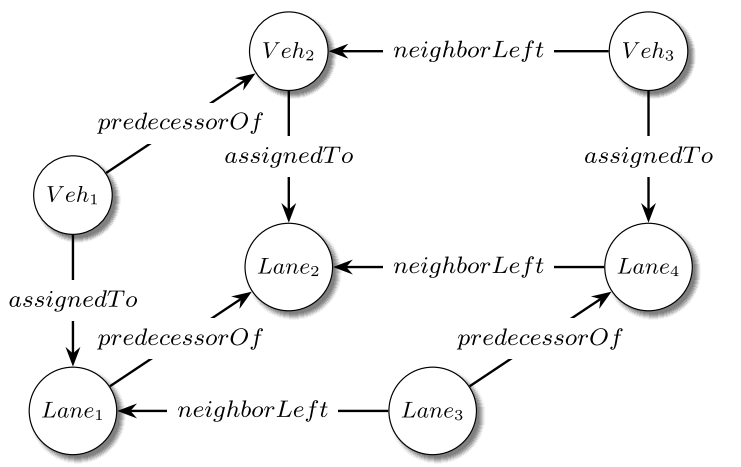
\includegraphics[width=0.5\linewidth]{98_images/relations}
	\caption[Semantic Relations between Traffic Participants]{Illustration of a Graph of Semantic Relations between Traffic Participants \cite{Petrich2018}}
	\label{fig:relations}
\end{figure}

\subsection{Principles of Dynamic World Modeling}
\label{subsec:concept_design:principle_of_dynamic_world_modeling}

\begin{samepage}
	Modeling road traffic requires the ability to capture and integrate perceptual information of highly dynamic environments properly – a problem for which \cite{Crowley1993} states five essential principles. In the following, the original term \textit{"'primitive"'} is substituted by \textit{"'entity"'}. 
	
	\begin{enumerate}[\ \ P1:]
		\item Entities in the world model should be expressed as a \textbf{set of properties}.
		\item Observation and model should be expressed in a \textbf{common coordinate system}.
		\item Observation and model should be expressed in a \textbf{common vocabulary}.
		\item Properties should include an \textbf{explicit representation of uncertainty}.
		\item Entities should be accompanied by a \textbf{confidence factor}.
	\end{enumerate}
\end{samepage}

This principles are picked up again for the concrete model specification presented later.

\cite{Crowley1993} also presents a "'General Framework for Dynamic World Modeling"', depicted in \autoref{fig:dynamic_world_modeling} (left). It illustrates the high-level process to transform heterogeneous types of observations into a unified model using a common vocabulary. The process includes a \textit{Match-Update-Predict} cycle, the purpose of which is to enhance observations with evidence derived from previous observations and a prediction model. Although especially the \textit{Match} step is quite essential for a real-world system, it is neglected in this thesis for the sake of focusing on the higher-level system architecture. Instead, a simplified process (right) is applied.

Throughout the course of following sections, the above principles are referenced using the respective \textit{\textbf{P}} prefixes.

\begin{figure}
	\centering
	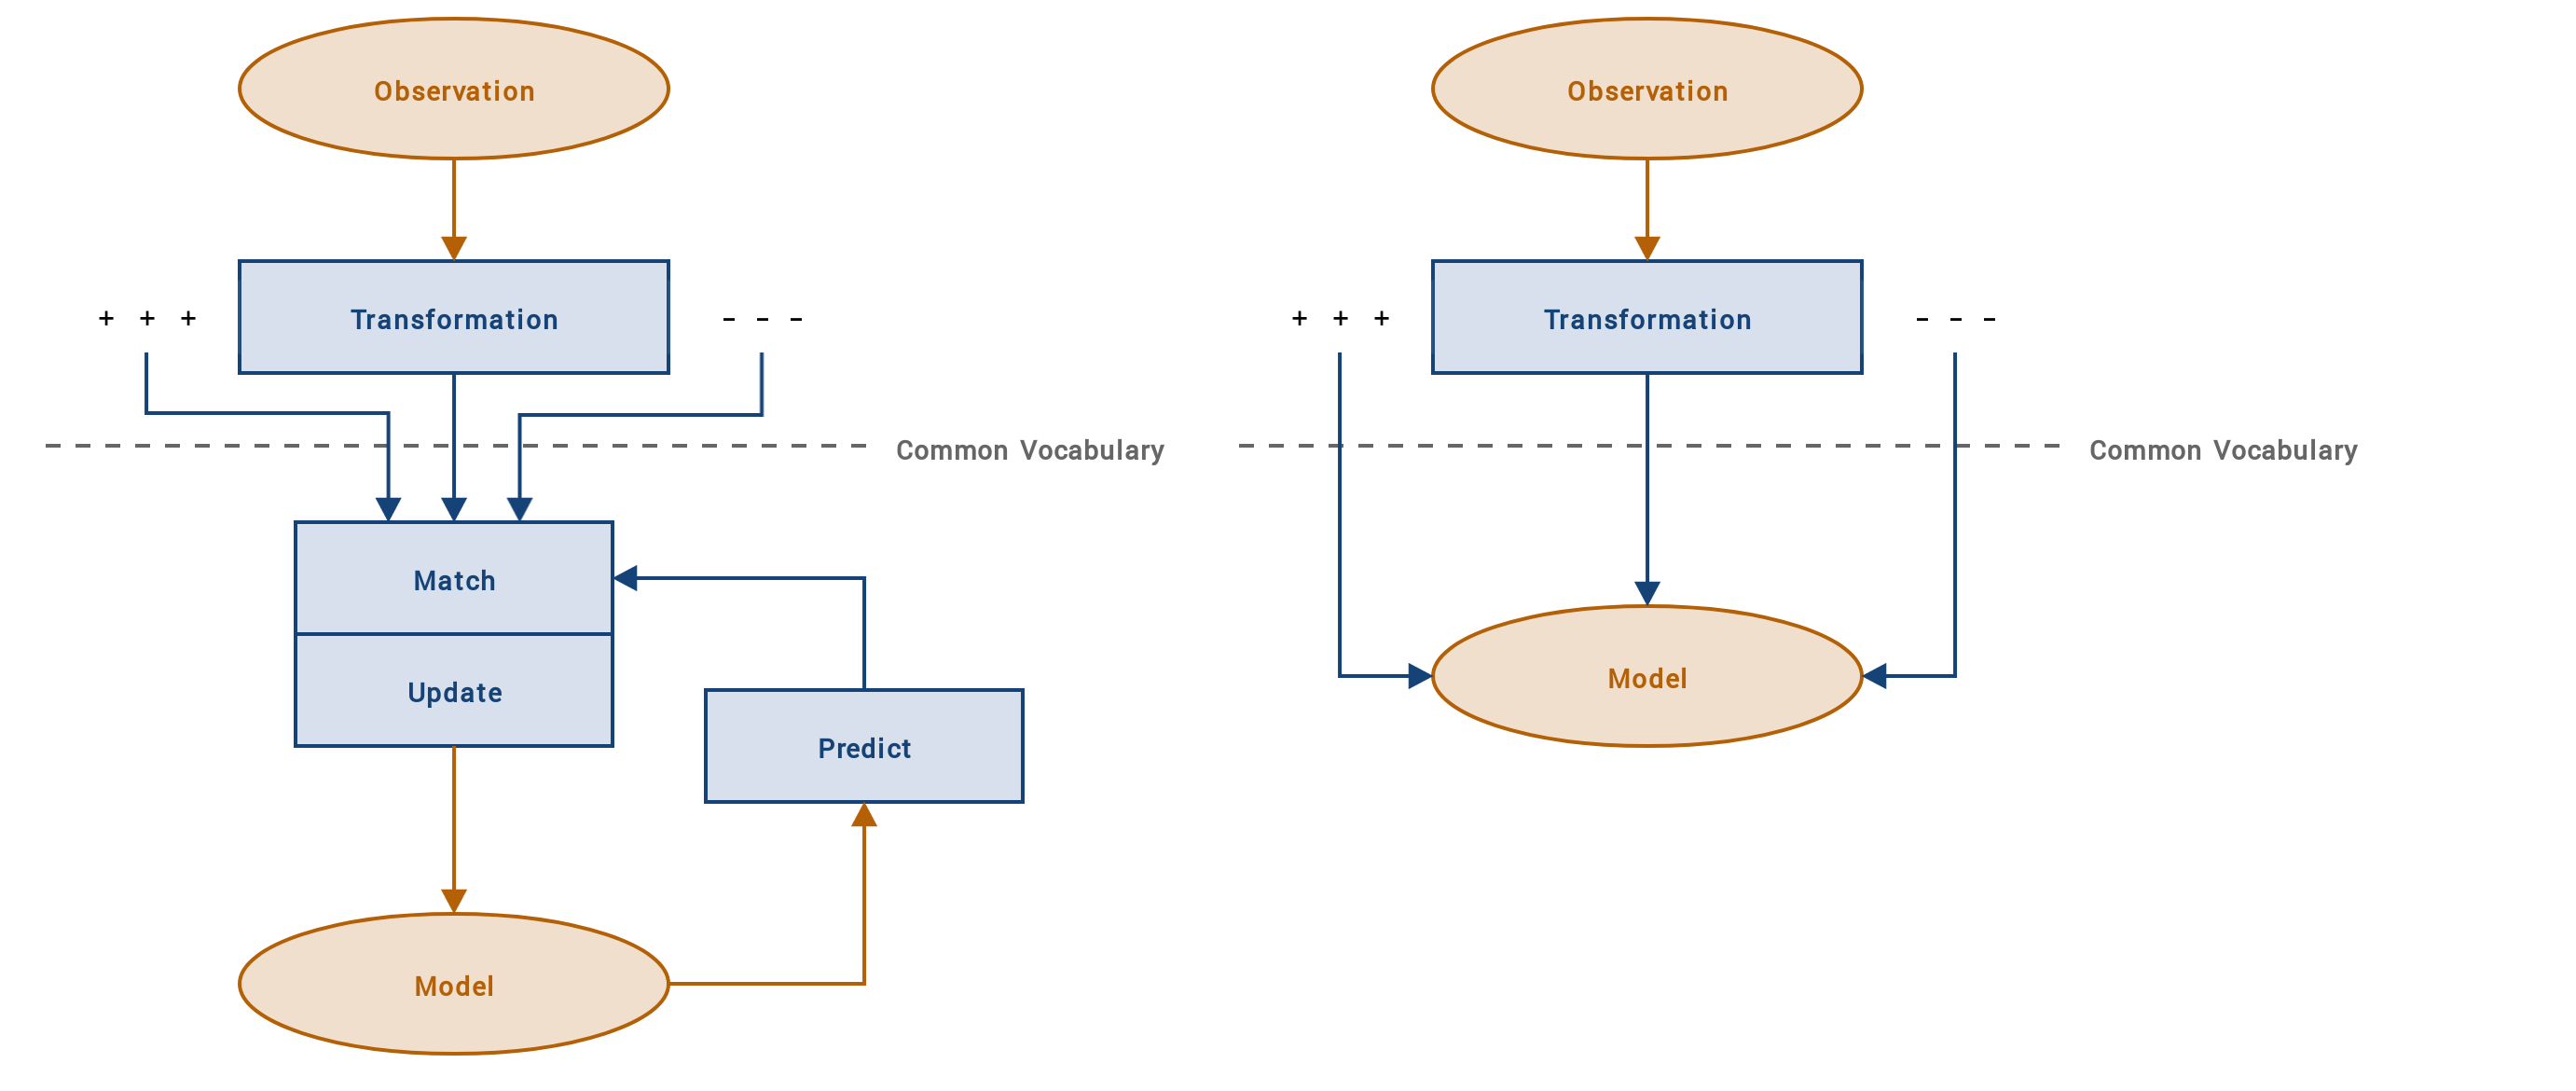
\includegraphics[width=1.0\linewidth]{98_images/dynamic_world_modeling}
	\caption[General Framework for Dynamic World Modeling]{General Framework for Dynamic World Modeling \cite{Crowley1993} (left: original, right: simplified version used in this thesis)}
	\label{fig:dynamic_world_modeling}
\end{figure}

\subsection{Discrete Environment Model with Occupancy Tiles}
\label{subsec:concept_design:discrete_environment_model_with_occupancy_tiles}

When attempting to model one's neighboring traffic environment, a mental distinction can be made into modeling the road network – including lane topology, traffic lights, sidewalks, etc. – and modeling static and dynamic obstacles, like other vehicles, pedestrians or trees. Both aspects are needed for a complete representation, as it is neither sufficient to only know the course of the road nor to only be aware of obstacles. Moreover, it is not sufficient to solely know an obstacle's position, but instead one is usually interested in more advanced properties, too. This work aims to combine all of these aspects in a shared model to enable them for being perceived cooperatively. Accordingly, the idea of \cite{Rauch2011} to share an object list is combined with the concept of \cite{liu2013motion} to share a discretized driveability map, also known as \textit{occupancy grid}. 
\par
\bigskip

The very base of our proposed model is made up of cells of an \textbf{occupancy grid} with fixed dimensions. Such can be constructed by any observer (vehicle, RSU, etc.) and derived from any kind of perceptual sensor data. This simplification facilitates universality \textbf{(NF-M1)}. However, these basic information can be enriched with more complex features easily to support expressiveness \textbf{(F-M1)}. This is achieved through the use of a graph-based meta model, as explained in \autoref{subsec:concept_design:probabilistic_entity_relationship_model_for_cooperative_perception}.

To work towards the perspicuity \textbf{(NF-M2)} requirement and to follow the principle of using a common coordinate system (\textbf{P2}), every cell is identified by a \textbf{QuadKey}. As a consequence, referring to a cell's position is independent from local, per-vehicle coordinates systems and from the GNSS / GPS coordinate frames alike. This prevents network participants from a multitude of expensive transformation operations.

Following this concept, the entire world map is recursively split into QuadTiles (see \autoref{sec:background:geo_tiling}) of a certain precision level (e.g. level 24, corresponding to square tiles of \textasciitilde\SI{2.39}{\square\meter}). The precision level should be chosen in a way that it is fine-grained enough to distinguish between single pedestrians or even road signs. However, at the same time, it must not be too exact to save bandwidth and computation load.

Each cell of the occupancy grid – one of which is observed locally by every connected participant – then corresponds to a certain QuadTile. Besides its occupancy state, every tile can be augmented with information like the corresponding occupant actor, its relation to the overall road topology, etc. 

\autoref{fig:tiling1} illustrates the proposed \textit{occupancy tile} concept. The blue grid is within the observation range of the turquoise vehicle and inherently part of larger tiles. Each cell's (= each tile's) state is determined through local sensor fusion involving different types of in-vehicle sensors and can be extended by additional information. Eventually, that grid, entailing all relevant information, is shared with other CP participants.

\begin{figure}[h]
	\centering
	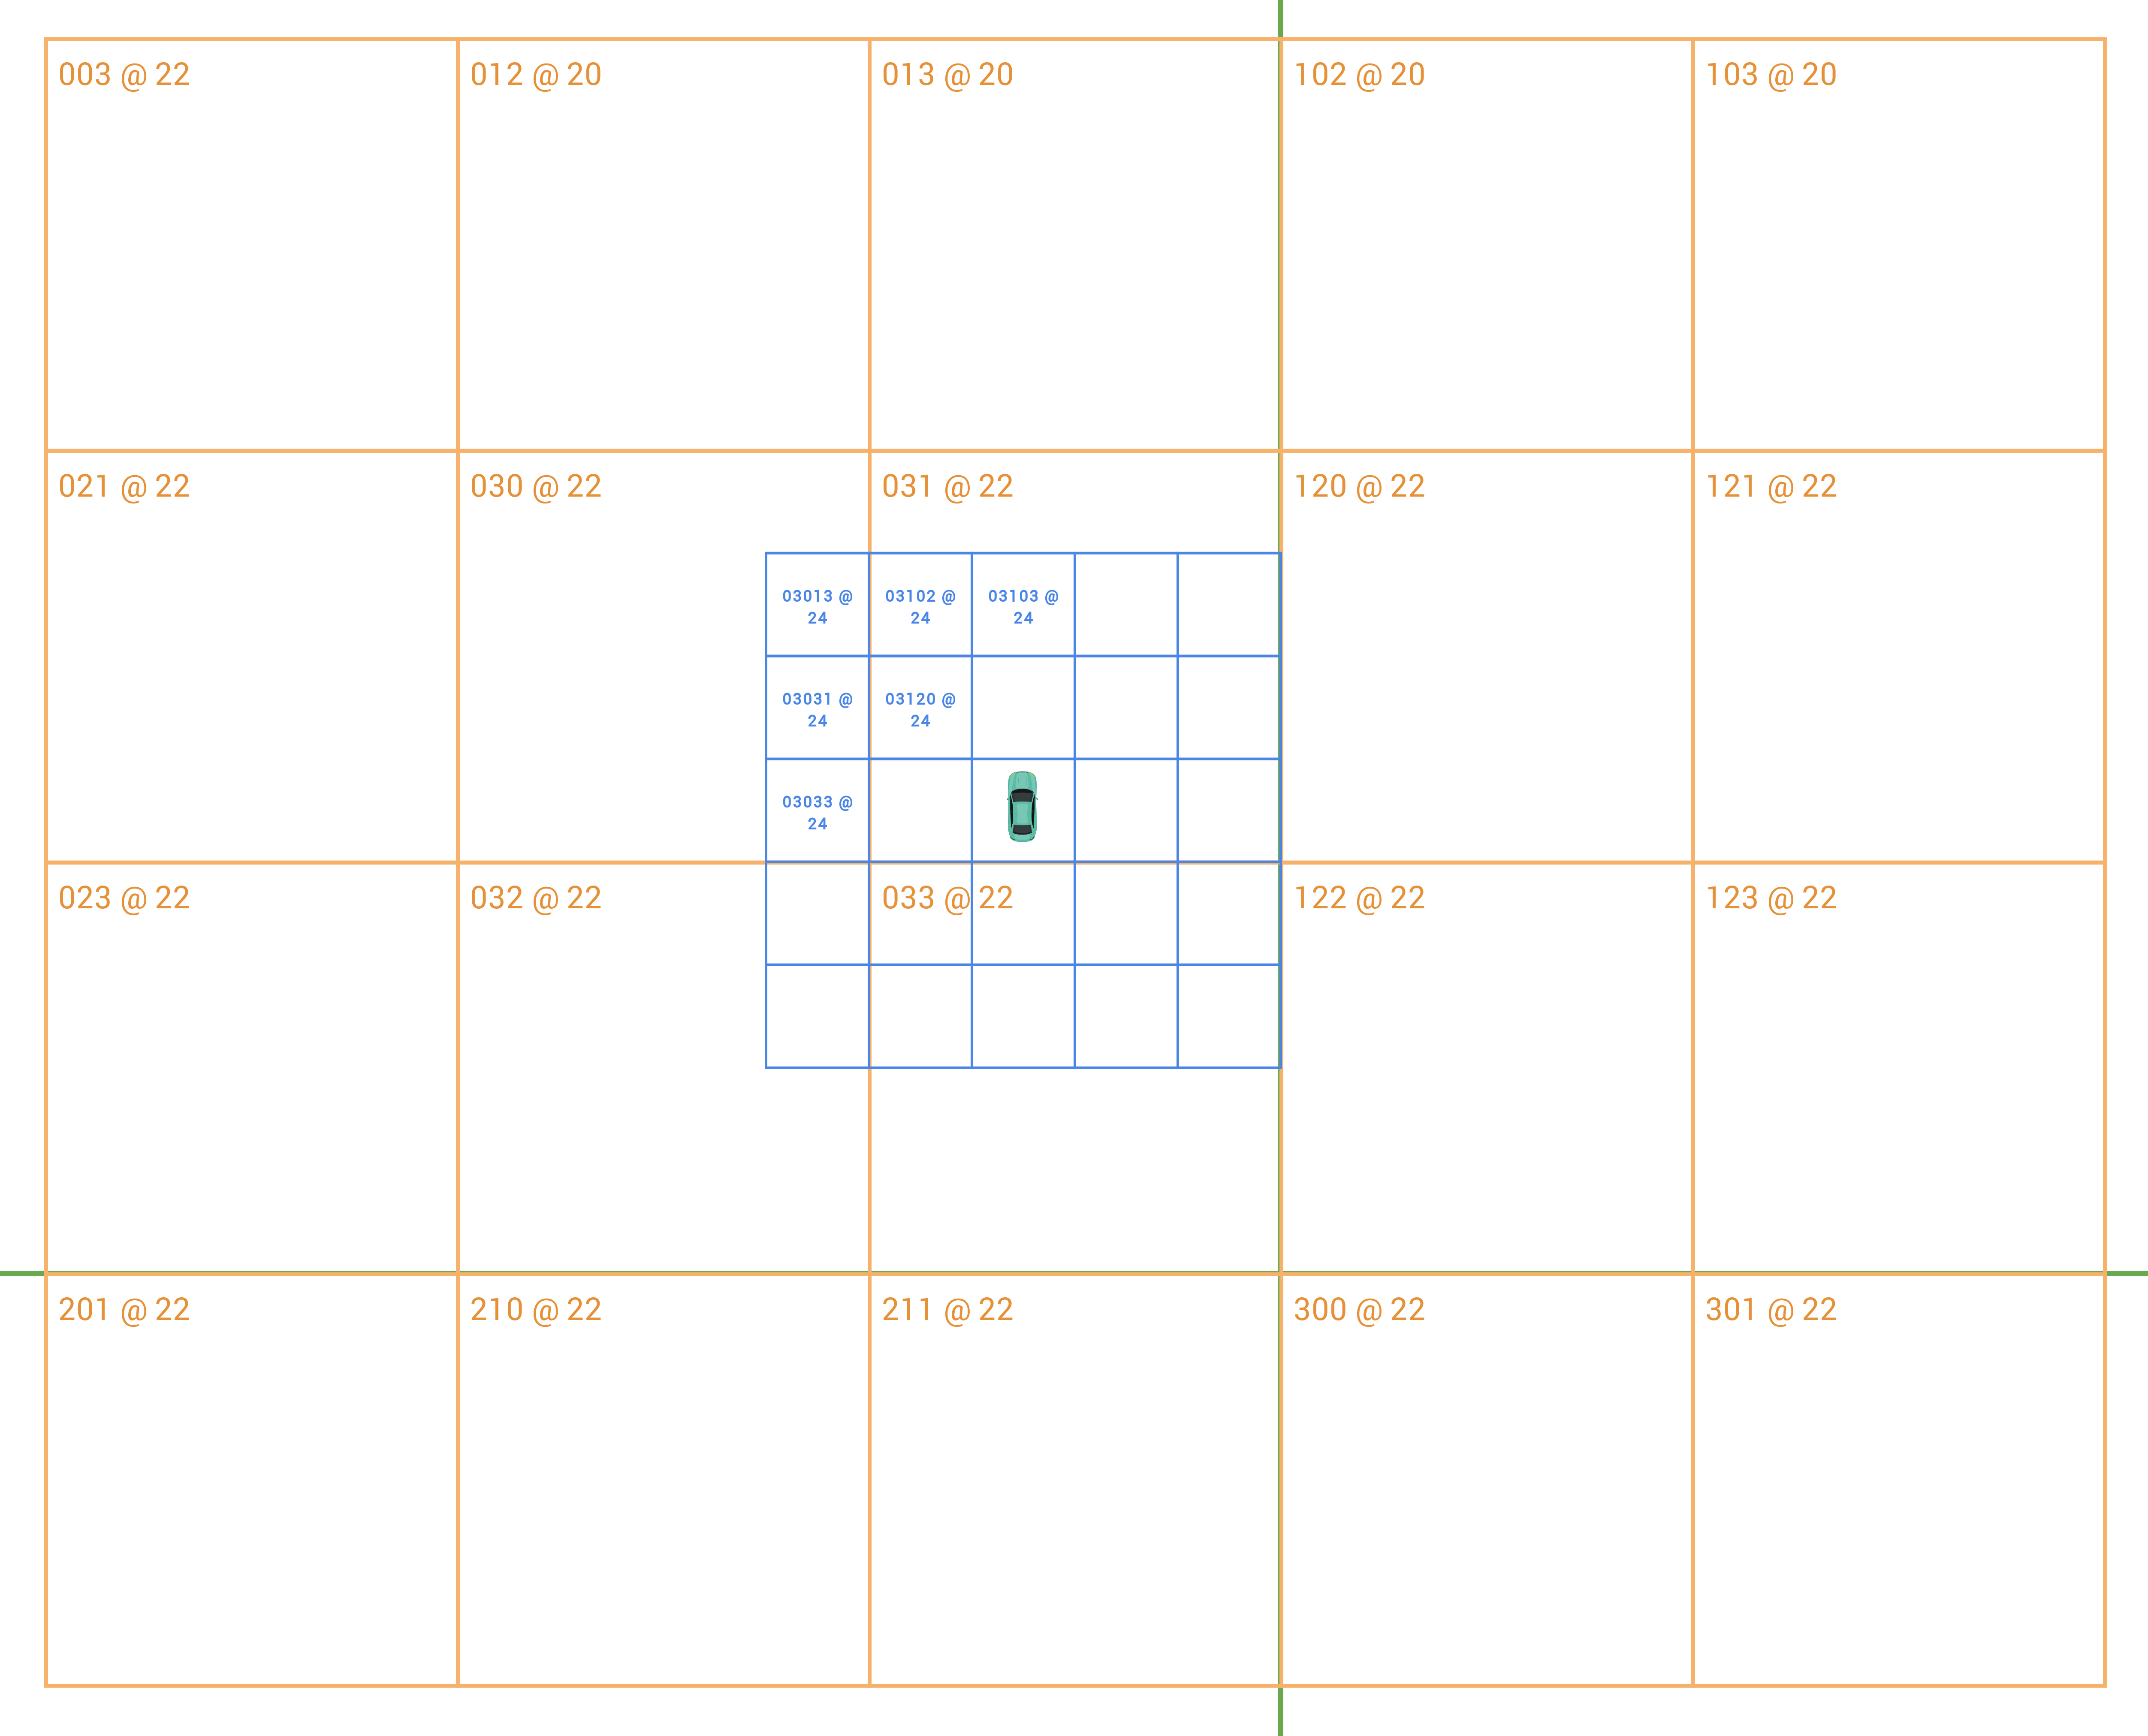
\includegraphics[width=1.0\linewidth]{98_images/geo_subscription_schema_1}
	\caption{Illustration of an Occupancy Grid using QuadTiles}
	\label{fig:tiling1}
\end{figure}


\subsection{Probabilistic Entity Relationship Model for Cooperative Perception}
\label{subsec:concept_design:probabilistic_entity_relationship_model_for_cooperative_perception}

In the simplest case, each observed cell of the previously introduced occupancy holds only information on whether it is occupied or not. However, this binary piece of data is usually insufficient to extensively describe a road scene. In addition, object-level static- (e.g. type, color and extent) and dynamic (e.g. velocity- and acceleration) information are desirable, e.g. about the occupying obstacle. This is in line with the requirements to support expressiveness \textbf{(F-M1)} openness \textbf{(F-M2)} and can be taken even one step further. To do so, \cite{Kohlhaas2014, Petrich2018} motivate the idea to also include high-level semantic information about the relationships between different entities in a scene to reduce complexity and help generalization. 

Up to this point, it is coarsely specified \textit{what} to incorporate into the model: static and dynamic properties of each entity within the scene on different levels of abstraction – including semantics – using occupancy tiles as base- or root entities. The second step is to specify \textit{how} to represent these. Previous requirements imply a structure in which \textbf{entities} have \textbf{attributes} (or properties, see principle \textbf{P1}) and \textbf{relations} of various types among different entities can exist. Additionally, in order to appropriately meet the inherently uncertain nature of a partially observable environment using imperfect sensory and to comply with principles \textbf{P4} and \textbf{P5}, some notion of \textbf{confidence} needs to be incorporated into the model. A way is needed to probabilistically model an observer's belief in the truthfulness of a particular property value or the existence of a certain relation between entities. 

These needs lead to the introduction of \textbf{Probabilistic Entity Relationship Models} (PER models). Such are already used by \cite{Petrich2018} for traffic scene representation and can be seen as an extension to regular Entity Relationship Models (ER models). Correspondingly, they incorporate the notion of entities with attributes and inherently define entity-entity relations. Both entity-attribute combinations and entity-entity relations can be represented as $\langle subject, predicate, object \rangle$ triples:

$$r \in \{ \langle \mathcal{E} \times \mathcal{A} \cup \mathcal{R} \times \mathcal{E} \cup \mathcal{L} \rangle \}$$

$\mathcal{E}$ is the set of all entities, $\mathcal{A}$ is the set of all attributes, $\mathcal{R}$ is the set of all entity-entity relations and $\mathcal{L}$ denotes a literal, i.e. a number, boolean value or string.

With PER models, every triple is extended with an additional confidence parameter and thus becomes a \textbf{quadruple} $r$ of $\langle subject, predicate, object, \textit{conf} \rangle$: 

\begin{gather*}
	r \in \{ \langle \mathcal{E} \times \mathcal{A} \cup \mathcal{R} \times \mathcal{E} \cup \mathcal{L} \times \Gamma \rangle \} \\
	\text{with} \  \Gamma := \{ \gamma \in [0, 1] \subset \mathbb{R}^+ \} \\
\end{gather*}

\cite{Petrich2018} distinguishes between \textit{attribute-} and \textit{structure uncertainty}, where the first describes sensor noise and the latter reflects uncertainty in the relational data. This is analogous to principles \textbf{P4} and \textbf{P5}, which suggest to model uncertainty for properties on the one hand and a confidence factor for entities on the other. However, this distinction is not considered useful in the context of this work and thus both probabilities are subsumed under a single notion of confidence.

An exemplary excerpt from an instantiated PER model, that was constructed based on observations of some ego vehicle, might look like this:

\begin{gather*}
	\langle \textit{obstacle\_25}, \textit{isOfType}, \textit{"'small\_car"'}, 0.921 \rangle \\
	\langle \textit{obstacle\_25}, \textit{hasVelocity}, (0.65, 0.42, 0), 0.448 \rangle \\
	\langle \textit{obstacle\_25}, \textit{isStoppedAt}, \textit{traffic\_light\_190}, 0.995 \rangle
\end{gather*}

In the example, $\textit{obstacle\_25}$ and $\textit{traffic\_light\_190}$ are entities, which were perceived, identified and tracked by an intelligent vehicle's sensory. $\textit{isOfType}$ and $\textit{hasVelocity}$ are attribute relations with attributes literals (string and three-dimensional numeric vector) and $\textit{isStoppedAt}$ stands for an entity-entity relation.

Such relations can be separated into seven classes: \textit{inclusion}, \textit{possession}, \textit{attachment}, \textit{attribution}, \textit{antonym}, \textit{synonym} and \textit{case} \cite{Storey1993}. Three of those are considered relevant for modeling in AD contexts \cite{Petrich2018}.

\begin{itemize}
	\item \textbf{Inclusion:} Indicates structural- or spatial inclusion or class inheritance. \\ Example: $\langle  cross\_walk\_12, isPartOf, lane\_30, \gamma \rangle$
	\item \textbf{Attachment:} Indicates structural- or spatial connection or intersection. \\ Example: $\langle car\_1250, drivesOn, lane\_30, \gamma \rangle$
	\item \textbf{Case:} Indicates interaction or dependence between entities or association of attributes and entities. \\ Examples: $\{ \langle car\_1250, isStoppedAt, traffic\_light\_190, \gamma \rangle, \langle bicycle\_370, hasColor, \\ "'yellow"', \gamma \rangle \}$
\end{itemize}

While relations from any of these classes are represented equally in an PER model, the distinction can help to achieve a clean meta model or database design.
\par
\bigskip

Using quadruples, a PER model is representable as a graph and thus can quite easily be searched, transformed and extended by inserting new relations. Also, the PER can – under certain conditions – be efficiently (\textbf{NF-M3}) represented as a tensor \cite{Petrich2018}.

The graphical representation also allows for different types of inference. New facts about the local world could be inferred when used in combination with first-order logic. Also, situations might easily be compared in terms of similarity, which can be used for case-based reasoning. \cite{Nickel2016} presents a multitude of further techniques to perform relational machine-learning on knowledge graphs, which might prove promising in AD contexts as well. 

\subsection{The Final Model}
\label{subsec:concept_design:the_final_model}
The complete model proposed as part of this thesis is presented in \autoref{fig:final_model}. It aims to be sufficiently comprehensive and includes all aspects needed for an in-depth evaluation of cooperative perception. However, the presented version is still not 100 \% complete. Future work in cooperation with expert groups is desirable to further extend it. 

In the illustration, blue boxes denote entities, orange boxes stand for uncertain entity-entity relations and green circles are uncertain attributes (or entity-literal relations). Gray boxes are special in a way that they can not be subject to instantiation, but rather define the meta model's static structure as a class hierarchy. Filled blue boxes are not of a special meaning, except that they usually occur particularly frequently.

In an instantiation of this model, quadruples include entities (blue) as subject or as subject and object and relations (orange) or attributes (green) as predicate. 

It is worth noting that, in contrast to most prior work in this field, the occupancy state of a cell is modeled \textbf{ternary} instead of binary. An additional bit is used to distinguish between a cell being \textit{free} or \textit{occupied} or just \textit{unknown}. This distinction adds valuable information for the participants of CP network, as an  \textit{unknown} (or \textit{unseen}, \textit{covered}, \textit{beyond-LOS}) state can simply be substituted during the fusion step. In a situation where two vehicles are driving in line (depicted in \autoref{fig:blocked_los_scenario}), the rear car might observe the cells occupied by the leader as occupied. However, there is no chance it can see through the leader car and thus all cells in front of it need to be communicated as being unknown, as opposed to either free or occupied.

\begin{figure}[h]
	\centering
	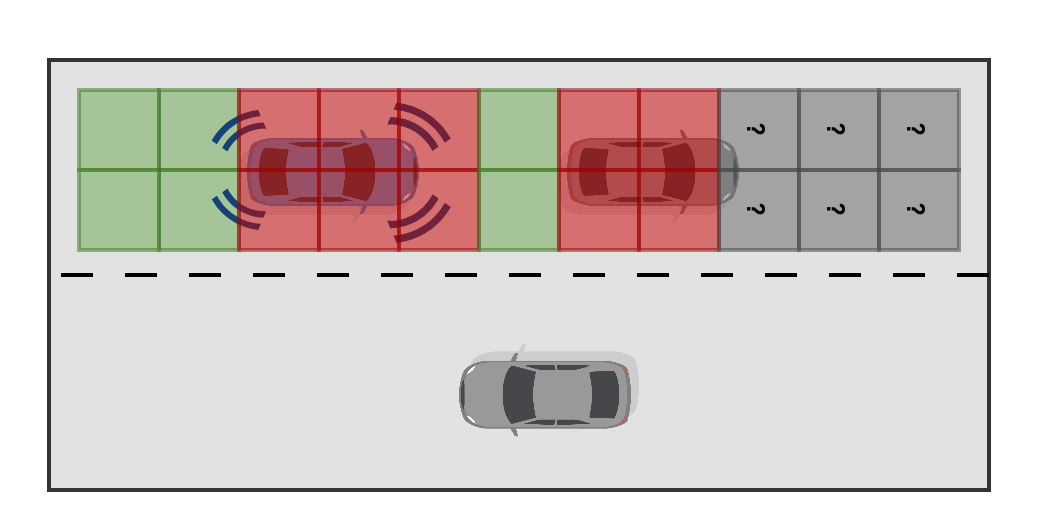
\includegraphics[width=0.7\linewidth]{98_images/unknown_cells_scene}
	\caption{Blocked Line of Sight Scenario}
	\label{fig:blocked_los_scenario}
\end{figure}


In addition, the presented model is rich in a way that ...

\begin{samepage}
	\begin{itemize}
		\item ... it defines a large variety of different entities and relations.
		\item ... it allows to exhaustively specify a cell's occupancy state.
		\item ... features different levels of abstraction (low-level attributes, high-level semantic relations).
		\item ... incorporates class hierarchies as known from object-oriented programming (e.g. $\langle Vehicle, isA, DynamicObstacle \rangle$).
	\end{itemize}
\end{samepage}

A minimal instantiation of this model has to include an \textit{OccupancyGrid} instance with an observer (\textit{observedBy}) \textit{Element} (e.g. a \textit{Vehicle}) and  $1..n$ \textit{GridCells}. How many cells exactly a grid consists of (grid size) can be configured and depends on its observer's sensor range. Each cell has to have at least its \textit{state} and \textit{positionHash} (as a QuadKey) defined. The ternary state can be represented using two bits, its \textit{positionHash} fits into 64 bits when using a QuadKey's integer representation (see \autoref{subsec:background:quadkeys}) and the confidence $\gamma$ would usually be implemented as a 32-bit float. Accordingly, one cell could be modeled using 98 bits in an optimal, minimalist case, what contributes to efficiency (\textbf{NF-M3}).

\begin{sidewaysfigure}
	\centering
	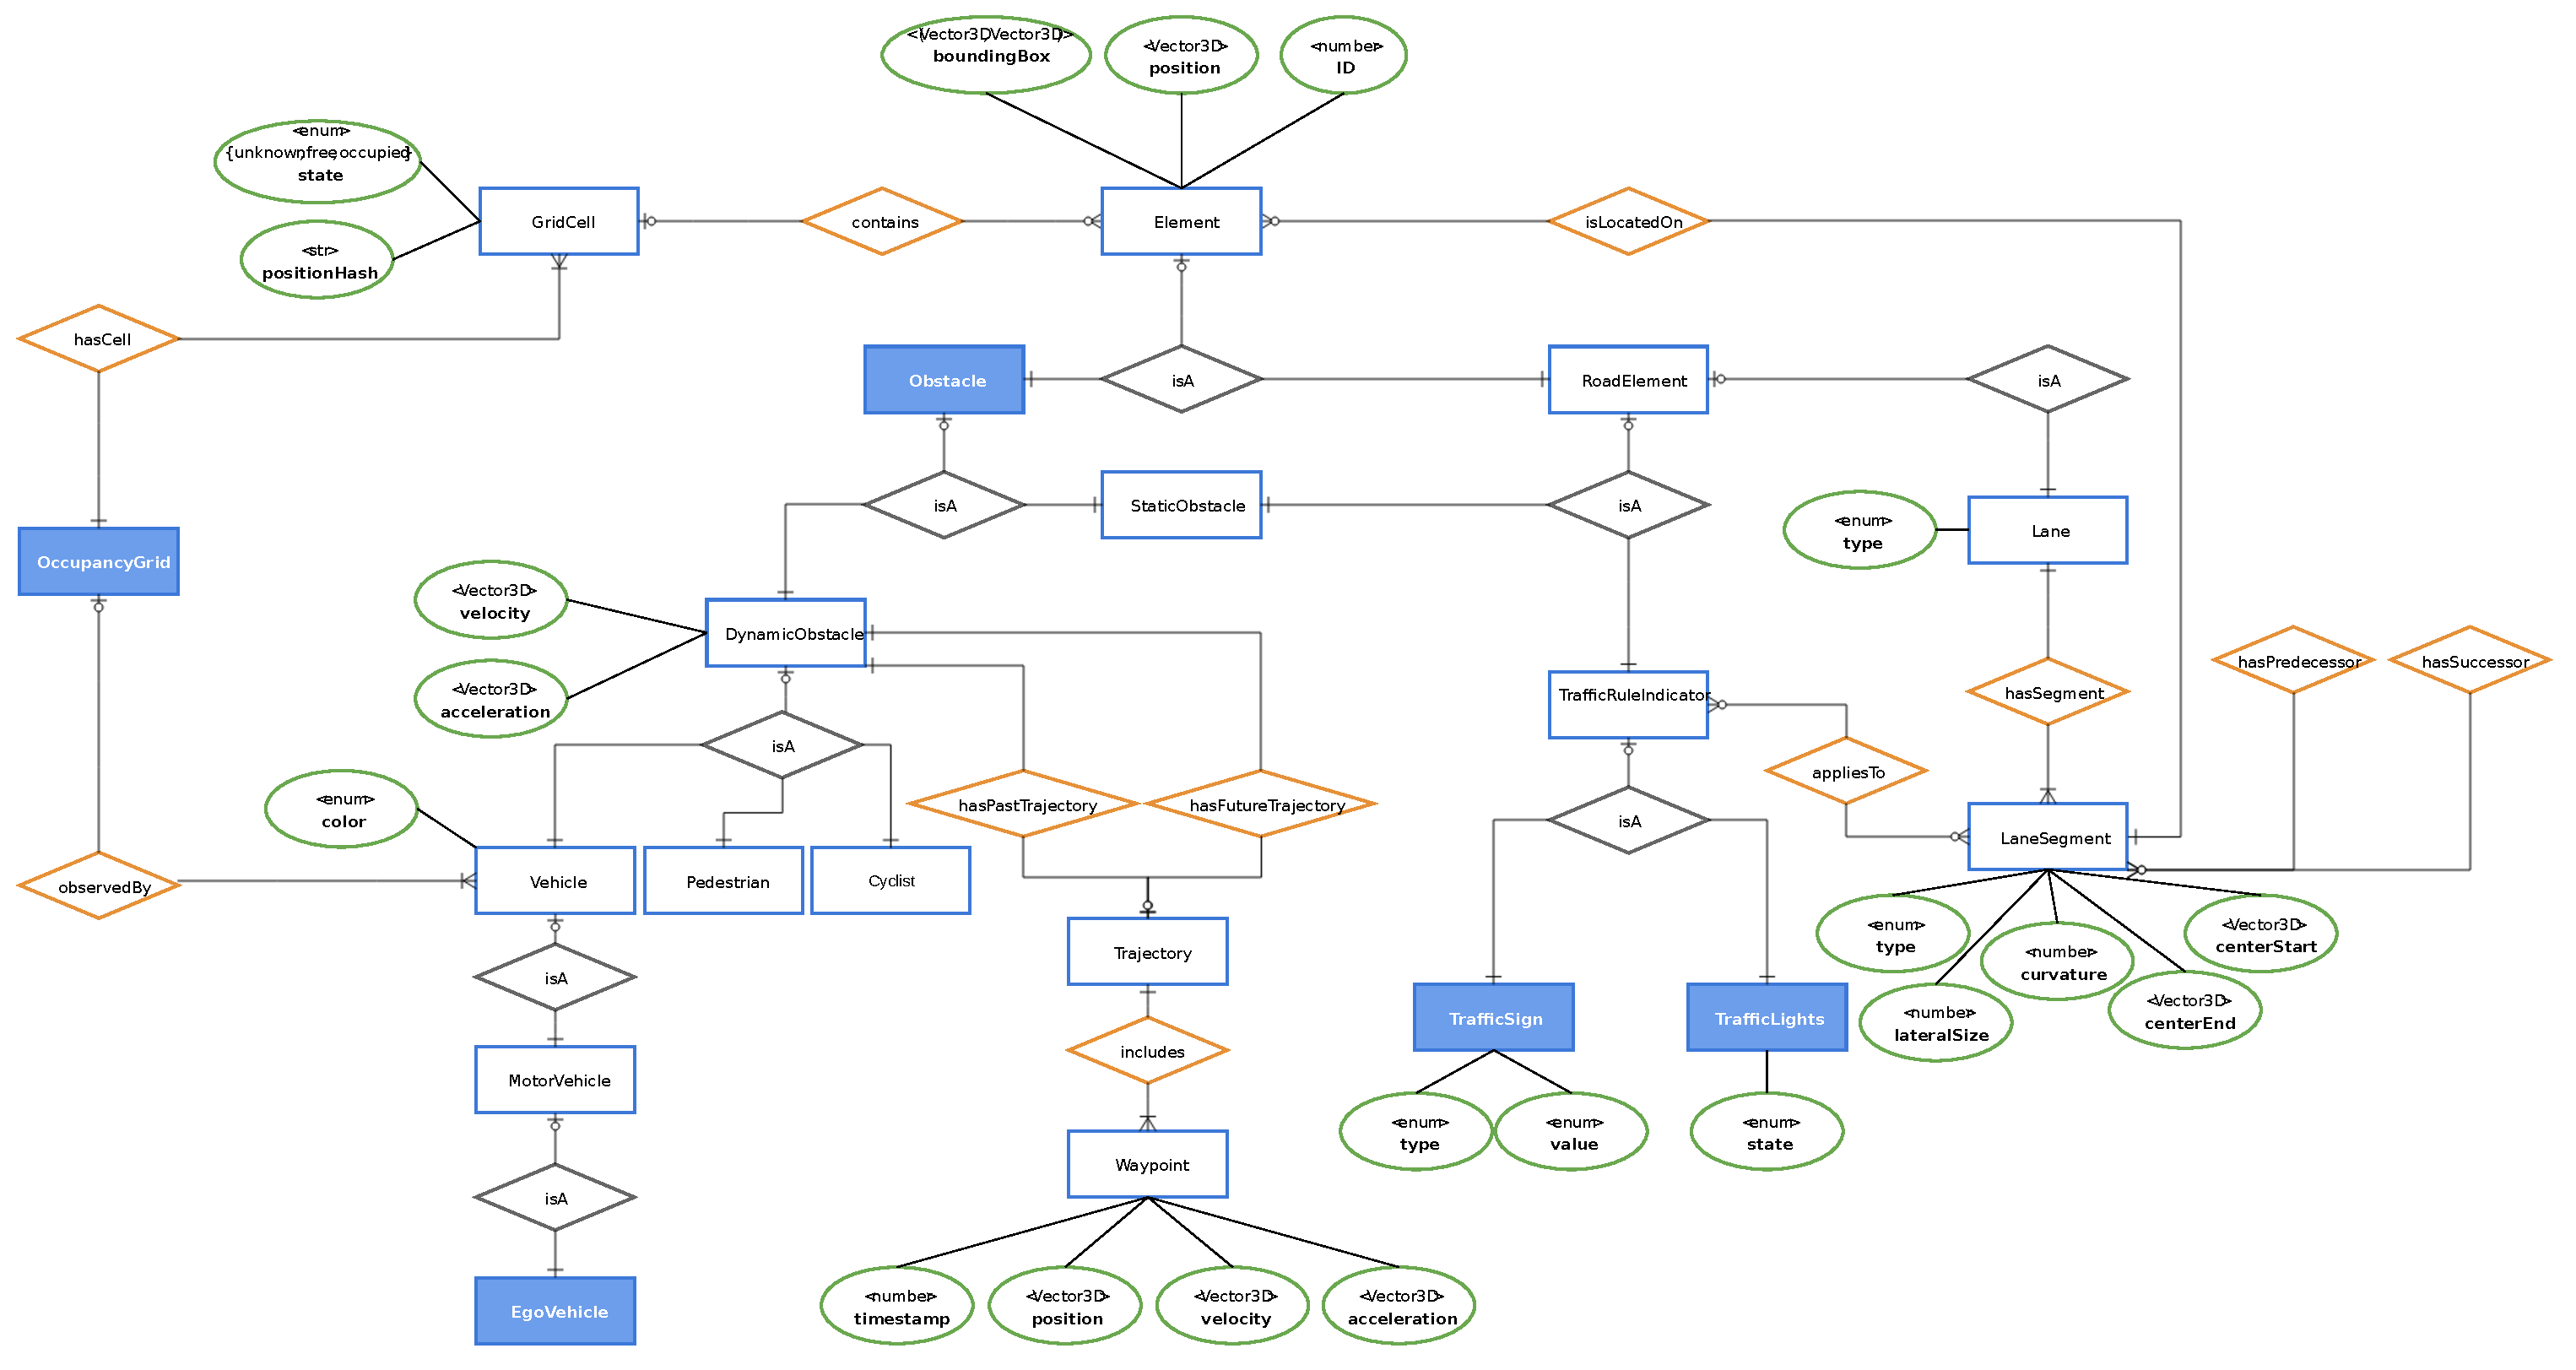
\includegraphics[width=\linewidth]{98_images/scene_representation_er}
	\caption{Comprehensive PER Model for Traffic Scenes}
	\label{fig:final_model}
\end{sidewaysfigure}

\subsection{Summary}
\label{subsec:concept_design:modeling:summary}
In the previous sections a comprehensive, yet not complete, model for dynamic traffic scenes and with a focus on cooperative perception use cases was presented (see \autoref{fig:final_model}). It fulfills the requirements stated in \autoref{sec:problem_analysis:goals_requirements} and follows the modeling principles introduced in \autoref{subsec:concept_design:principle_of_dynamic_world_modeling}.

As a result, it is capable of uniformly and universally modeling road scenarios at a high degree of expressiveness, while embracing a notion of uncertainty or confidence and information on different abstraction levels. Key concepts used include \textbf{Geo tiling} – based on \textbf{QuadKeys} – for spatially referencing cells of an \textbf{occupancy grid} and \textbf{Probabilistic Entity Relationship models} as a structural framework.

\section{Cellular Communication}
\label{sec:concept_design:cellular_communication}
Various downsides of DSRC-based ad-hoc networks for cooperative perception use cases were already discussed in \autoref{sec:problem_analysis:limitations_of_prior_work}. They include issues arising from limited throughput and comparatively short range of IEEE 802.11p and similar technologies. Furthermore, P2P topologies usually imply a large communication overhead and result in high computational load for each participant. To overcome these limitations, an alternative approach is proposed that builds on 5G networks and a client-server topology.

This section briefly presents characteristics, key benefits and implications of 5G technology for V2X communication and motivates the decision for its use in the present CP system.

\subsection{5G Characteristics \& Advantages}
\label{subsec:concept_design:5g_characteristics_advantages}
5G stands for the fifth generation cellular network standard and is the successor of 4G, or LTE. It may be operated on a variety of different spectrums, ranging from low-band (\textasciitilde 600 Mhz) over mid-band (2.4 to 4.2 \si{\giga\hertz}) to millimeter waves in the high-band spectrum ranging from 24 to 72 \si{\giga\hertz}. Which spectrum is used depends mainly on the character and has direct influence on communication range and speed.

In networks based on the most widely used mid-band spectrum, average throughput is between 100 and 400 \si{\mega\bit\per\second}, while it can increase up to \SI{2}{\giga\bit\per\second} with millimeter waves \cite{wiki:5g}.

Typical round-trip (RTT) were measured to range from 25-35 \si{\milli\second} and might be improved to 10-20 \si{\milli\second} when employing an \textit{Edge Node} (see \autoref{sec:background:edge_computing}) close to a cell tower \cite{wiki:5g}. Under lab conditions, even less than \SI{1}{\milli\second} latencies were observed.

According to \cite{Singh2018}, 5G networks allow up to \SI{900000}{vehicles\per\square\km} and they may have a speed of up to \SI{500}{\km\per\hour}.

Like 4G, 5G is based on network cells between which moving mobile clients are handed over. Generally, network cells are smaller with 5G than with 4G, especially in densely populated areas.

\cite{5GAutomotiveAssociation2016} presents a detailed, technical discussion of 5G vs DSRC for V2X, while a higher-level comparison with respect to key implications for CP is presented in \autoref{tab:5g_dsrc_comparison}.
\par
\bigskip

ETSI identified three different main usage scenarios for 5G \cite{ETSI5G}, all of which require different key capabilities, as shown in \autoref{fig:5g_capabilities}. The different usage scenarios are:

\begin{itemize}
	\item \textbf{Enhanced Mobile Broadband (eMBB)} to be used for high-definition, low-latency multimedia content and mobile games on end-user devices and smartphones.
	\item \textbf{Massive Machine-type Communications (mMTC)} for the Internet of Things, which is characterized by low-power devices and low data rates.
	\item \textbf{Ultra-reliable and Low Latency Communications (URLLC)} for safety- and mission-critical applications, like autonomous driving. 
\end{itemize}

Cooperative perception requires URLLC and thus especially low latency and high throughput.

\begin{figure}[h]
	\centering
	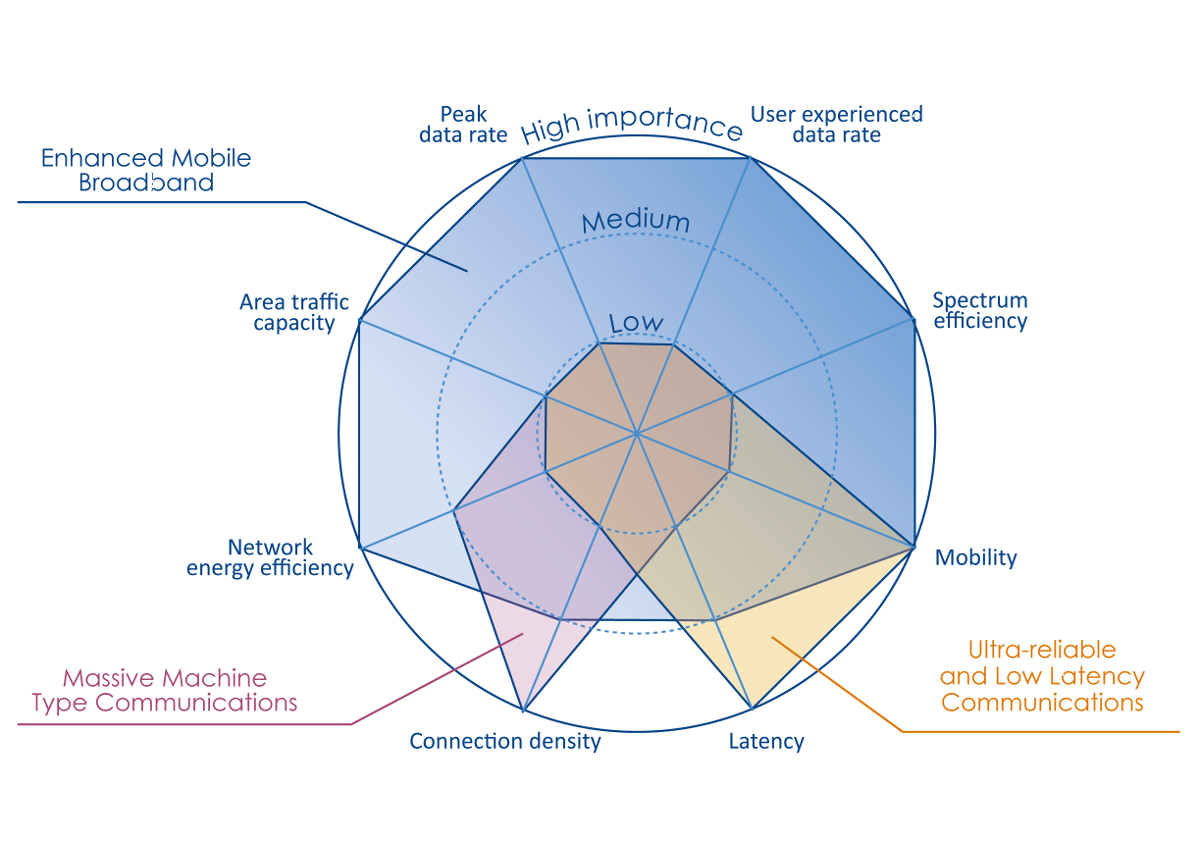
\includegraphics[width=0.75\linewidth]{98_images/5g_spider_chart}
	\caption[Key Capability Requirements for 5G]{Key Capability Requirements for 5G in different Scenarios \cite{ETSI5G}}
	\label{fig:5g_capabilities}
\end{figure}

\subsection{Vehicle-to-Network-to-Everything Communication Topology}
\label{subsec:concept_design:communication_topology}
Most prior work on V2X employs ad-hoc networks (VANETs) between participants, many of which imply a peer-to-peer network topology, i.e. every participant connects to every other participant, following \textit{Metcalfe's Law}. Downsides of such approaches were briefly outlined in \autoref{sec:problem_analysis:limitations_of_prior_work} and mainly refer to scalability and communication overhead.

In order to unburden participant vehicles (or pedestrian smartphones, RSUs, etc.), this work proposes the use of a \textbf{client-server architecture}. Every client connects to a central server instance, that is responsible for its current geographical area, which performs all computation tasks (mainly high-level sensor data fusion) and is responsible for collecting and broadcasting their messages. While the server node has to be very strong in terms of computational capacity, every client now only has to maintain one bi-directional connection and process (e.g. fuse) messages from one sender. \autoref{fig:communication_topology} illustrates both patterns in a scenario of $n = 4$ vehicles. The pattern of V2X now becomes, strictly speaking, V2N2X, as an intermediate network is involved. However, for the sake of simplicity, the term \textit{V2X} will still be used to describe this new pattern. 

Although 5GAA specify multiple transmission modes for 5G \cite{5GAutomotiveAssociation2016} – including \textbf{direct communication} between network clients (V2V in the narrow sense ot the word) – this thesis focuses on V2N-based communication to best counter the previously mentioned drawbacks. 

\begin{figure}[h]
	\centering
	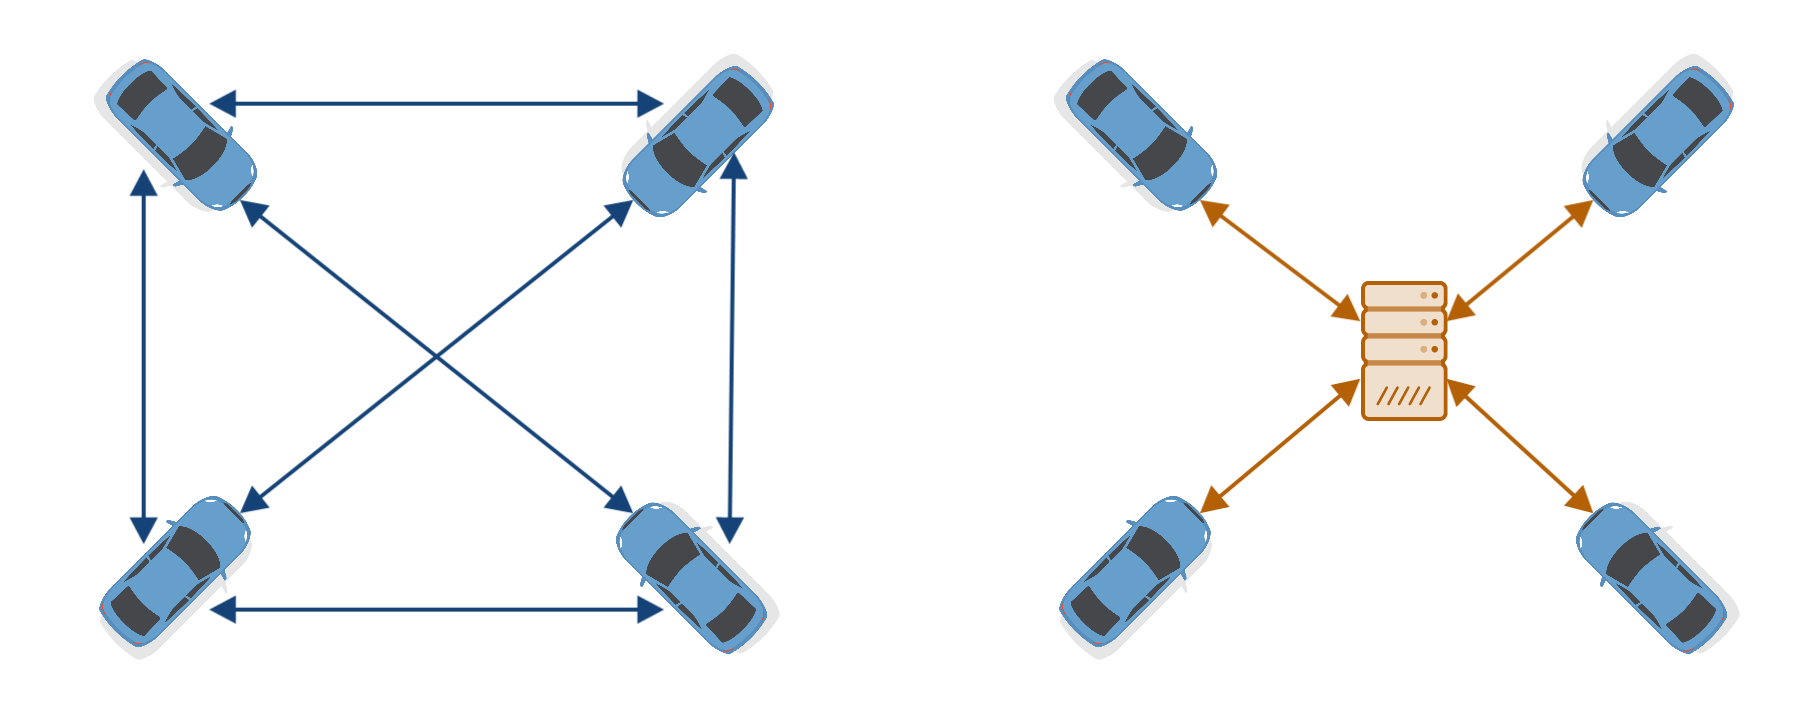
\includegraphics[width=0.9\linewidth]{98_images/topology_comparison}
	\caption{VANET vs. Client-Server Communication Topology}
	\label{fig:communication_topology}
\end{figure}


\subsection{Summary}
\label{subsec:concept_design:5g:summary}
In contrast to most prior work, the CP system developed in the context of this thesis does not rely on DSRC-based VANETs, but on cellular 5G communication with centralized server instances instead. Motivation for this decision was given in previous sections and is additionally summarized in \autoref{tab:5g_dsrc_comparison}.

\begin{table}[H]
	\begin{tabular}{|p{7.6cm}|p{7.6cm}|}
		\hline
		\textbf{VANETs + DSRC}                & \textbf{Client-Server + 5G cellular}                                                 \\ \hline
		\rowcolor[HTML]{9AFF99} 
		+ Works anywhere                      & \cellcolor[HTML]{FFCCC9}– Requires network infrastructure and -coverage              \\ \hline
		\rowcolor[HTML]{9AFF99} 
		+ Free of charge                      & \cellcolor[HTML]{FFCCC9}– Implies variable costs (e.g. data plan)                    \\ \hline
		\rowcolor[HTML]{9AFF99} 
		+ Network is solely dedicated for V2X & \cellcolor[HTML]{FFCCC9}– Potentially shared network, e.g. with end-user smartphones \\ \hline
		\rowcolor[HTML]{FFCCC9} 
		– Superlinear communication effort    & \cellcolor[HTML]{9AFF99}+ Linear communication effort                                \\ \hline
		\rowcolor[HTML]{FFCCC9} 
		– Linear computation effort for CP    & \cellcolor[HTML]{9AFF99}+ Constant communication effort for CP                       \\ \hline
		\rowcolor[HTML]{FFCCC9} 
		– 2.7-11 Mbps throughput \cite{Chen2016, Wang2013}              & \cellcolor[HTML]{9AFF99}+ \textgreater \ 65 Mbps throughput \cite{Kavanagh2019, wiki:5g}                          \\ \hline
		\rowcolor[HTML]{9AFF99} 
		+ 3-22 ms latency \cite{Rauch2011}                     & \cellcolor[HTML]{FFCCC9}– 10-20 ms latency (with Edge Node) \cite{wiki:5g, QualcommTechnologiesInc.2018}                          \\ \hline
		\rowcolor[HTML]{FFCCC9} 
		– $\sim$ 300 m NLOS range \cite{5GAutomotiveAssociation2018}              & \cellcolor[HTML]{9AFF99}+ $\sim$ 800 m NLOS range \cite{5GAutomotiveAssociation2018}                                     \\ \hline
		\rowcolor[HTML]{FFCCC9} 
		– P2P topology                        & \cellcolor[HTML]{9AFF99}+ P2P ("'direct communication"') or V2N topologies             \\ \hline            
	\end{tabular}
	\caption{Comparison of DSRC-based VANETs and 5G-based Client-Server V2X Networks}
	\label{tab:5g_dsrc_comparison}
\end{table}

In conclusion, 5G is a highly promising technology for cooperative perception and V2X communication in general. However, since it is a crucial requirement for the functioning of cellular V2X networks, their adoption will heavily depend on the market introduction of 5G. At the time of writing, 5G is still in its infancy. However, its expansion is being driven forward vigorously. For instance, German network operators are required to provide 5G coverage to 98 \% of all households by 2022 \cite{DeutscheWelle2019}. The authors of \cite{CCSInsight2018}, in turn, consider the market introduction of V2X applications an enabler for the establishment of 5G technology for mission-critical (URLCC, see \autoref{subsec:concept_design:5g_characteristics_advantages}) usage scenarios and estimate them to take off from 2025 on. However, they put the usage of 4G Advanced, or 4.5G, as a fallback mechanism in perspective.